%% LyX 2.1.3 created this file.  For more info, see http://www.lyx.org/.
%% Do not edit unless you really know what you are doing.
\documentclass[oneside,french]{amsart}
\usepackage[T1]{fontenc}
\usepackage{textcomp}
\usepackage{url}
\usepackage{tipa}
\usepackage{amsthm}
\usepackage{amstext}
\usepackage{amssymb}
\usepackage{graphicx}
\usepackage{esint}

\makeatletter
%%%%%%%%%%%%%%%%%%%%%%%%%%%%%% Textclass specific LaTeX commands.
  \theoremstyle{plain}
  \newtheorem*{lem*}{\protect\lemmaname}
  \theoremstyle{plain}
  \newtheorem*{prop*}{\protect\propositionname}

%%%%%%%%%%%%%%%%%%%%%%%%%%%%%% User specified LaTeX commands.
\renewcommand\[{\begin{equation}}
\renewcommand\]{\end{equation}}

\renewcommand{\labelenumi}{\emph{(\alph{enumi})}}

\renewcommand{\thefootnote}{\*} 

\makeatother

\usepackage{babel}
\makeatletter
\addto\extrasfrench{%
   \providecommand{\og}{\leavevmode\flqq~}%
   \providecommand{\fg}{\ifdim\lastskip>\z@\unskip\fi~\frqq}%
}

\makeatother
  \providecommand{\lemmaname}{Lemme}
  \providecommand{\propositionname}{Proposition}

\begin{document}

\title{Transform\'{e}e de scattering en spirale temps-chroma-octave}

\maketitle
Dans le cadre de la classification automatique de sons harmoniques,
on propose de remplacer l'axe fr\'{e}quentiel par une spirale faisant
un tour \`{a} chaque octave. On en d\'{e}duit une transform\'{e}e
en ondelettes \`{a} partir des d\'{e}placements \'{e}l\'{e}mentaires
sur la spirale. On donne une illustration num\'{e}rique des capacit\'{e}s
de discrimination de la transform\'{e}e en spirale \`{a} travers une
formulation transitoire du mod\`{e}le source-filtre. \footnote{Ce travail est financ\'{e} par la bourse ERC InvariantClass 32095.
Le code source des exp\'{e}riences et figures est en libre acc\`{e}s
sur \url{www.github.com/lostanlen/scattering.m}.}


\section{Du temps-fr\'{e}quence au temps-chroma-octave}

Les paradoxes de hauteur synth\'{e}tis\'{e}s par Shepard et Risset
{[}Risset{]} montrent que la perception de la hauteur n'est pas r\'{e}ductible
au continuum grave-aigu des fr\'{e}quences physiques. En effet, en
sommant des sinuso\"{\i}des de fr\'{e}quence $2^{n}f_{0}$ avec $n\in\mathbb{Z}$,
on obtient une note que l'on peut nommer sur une gamme musicale, bien
qu'elle ne puisse \^{e}tre localis\'{e}e dans le grave ou l'aigu.
D\`{e}s lors, en faisant progressivement cro\^{\i}tre $f_{0}$ jusqu'\`{a}
$2f_{0}$, on peut construire un \emph{glissando} qui semble monter
ind\'{e}finiment lorsqu'il est r\'{e}p\'{e}t\'{e}. Par ailleurs, en
filtrant les sinuso\"{\i}des dans une bande dont la fr\'{e}quence
centrale diminue, on peut donner l'impression de passer du registre
aigu au registre grave tout en restant sur la m\^{e}me note. La composition
de ces deux op\'{e}rations produit un son paradoxal qui monte localement
tout en descendant globalement. Cette exp\'{e}rience met en lumi\`{e}re
le fait qu'il y a en fait deux attributs perceptifs associ\'{e}s \`{a}
la fr\'{e}quence. Le premier, appel\'{e} hauteur tonale ou \emph{chroma},
encode la m\'{e}lodie musicale et l'intonation de la voix ; le second,
appel\'{e} hauteur spectrale ou simplement \emph{octave}, est une
composante essentielle du timbre.

Afin de prendre en compte ces propri\'{e}t\'{e}s, on choisit de remplacer
l'axe rectilin\'{e}aire des hauteurs par un sch\'{e}ma en spirale,
\`{a} raison d'un tour par octave : un changement de chroma est alors
analogue \`{a} une rotation, tandis qu'un changement d'octave est
une dilatation par rapport au centre de la spirale. Cette id\'{e}e
a \'{e}t\'{e} confirm\'{e}e par de nombreuses exp\'{e}riences en psychoacoustique,
mais aussi en neurologie de l'audition {[}Warren{]}. On verra \`{a}
la section 4 qu'elle permet d'interpr\'{e}ter une formulation transitoire
du mod\`{e}le source-filtre.

On commence par construire une transform\'{e}e en ondelettes couvrant
les fr\'{e}quences audibles : soit $\psi(u_{1})$ un filtre passe-bande
\`{a} valeurs complexes, de fr\'{e}quence centrale r\'{e}duite $1$
et de largeur de bande $1/Q$. L'analyse en ondelettes consiste \`{a}
dilater la transform\'{e}e de Fourier $\hat{\psi}(\omega_{1})$ de
$\psi(u_{1})$ par des facteurs de r\'{e}solution $\lambda_{1}>0$
: 
\[
\widehat{\psi_{\lambda_{1}}}(\omega_{1})=\hat{\psi}(\frac{\omega_{1}}{\lambda_{1}}),\;\text{c'est-\`{a}-dire}\;\;\psi_{\lambda_{1}}(u_{1})=\lambda_{1}\psi(\lambda_{1}u_{1}).
\]
La variable $\lambda_{1}$ est homog\`{e}ne \`{a} une fr\'{e}quence
(mesur\'{e}e en Hertz) relativement au temps $u_{1}$. Ainsi, chaque
ondelette $\psi_{\lambda_{1}}(u_{1})$ est un filtre passe-bande de
fr\'{e}quence centrale $\lambda_{1}$, de largeur de bande $\lambda_{1}/Q$
et de support temporel $Q/\lambda_{1}$. Son facteur de qualit\'{e},
d\'{e}fini comme le rapport de la fr\'{e}quence centrale sur la largeur
de bande, reste \'{e}gal \`{a} $Q$. On choisit $Q=16$ dans les figures
de cet article.

Un son de Shepard est une somme de sinuso\"{\i}des dont les fr\'{e}quences
s'\'{e}chelonnent sur des octaves cons\'{e}cutives. On peut les noter
$2^{k+\chi}$ avec $k$ parcourant $\mathbb{Z}$ et $\chi\in\left[0;1\right[$
une constante d\'{e}pendant du son de Shepard choisi. %ecrire que l'on peut toujours se restreindre au spectre audible donc pas de probleme d'integrabiliteOn
constate que les sons de Shepard ne peuvent pas \^{e}tre rang\'{e}s
selon un ordre lin\'{e}aire grave-aigu, mais doivent \^{e}tre agenc\'{e}s
en cercle.

Le scalogramme d'un son de Shepard vaut :
\[
x_{1}(u_{1},\lambda_{1})=\sum_{k=-\infty}^{+\infty}\delta(\lambda_{1}-2^{k+\chi})=\sum_{k=-\infty}^{+\infty}\delta(\log_{2}\lambda_{1}-k-\chi)
\]


s'\'{e}crivent $2^{k}\xi$ avec $k\in\mathbb{Z}$. Sur un axe log-fr\'{e}quentiel,
celles-ci s'\'{e}crivent 

%Commenter le scalogramme et motiver la spirale

\begin{figure}
\hfill{}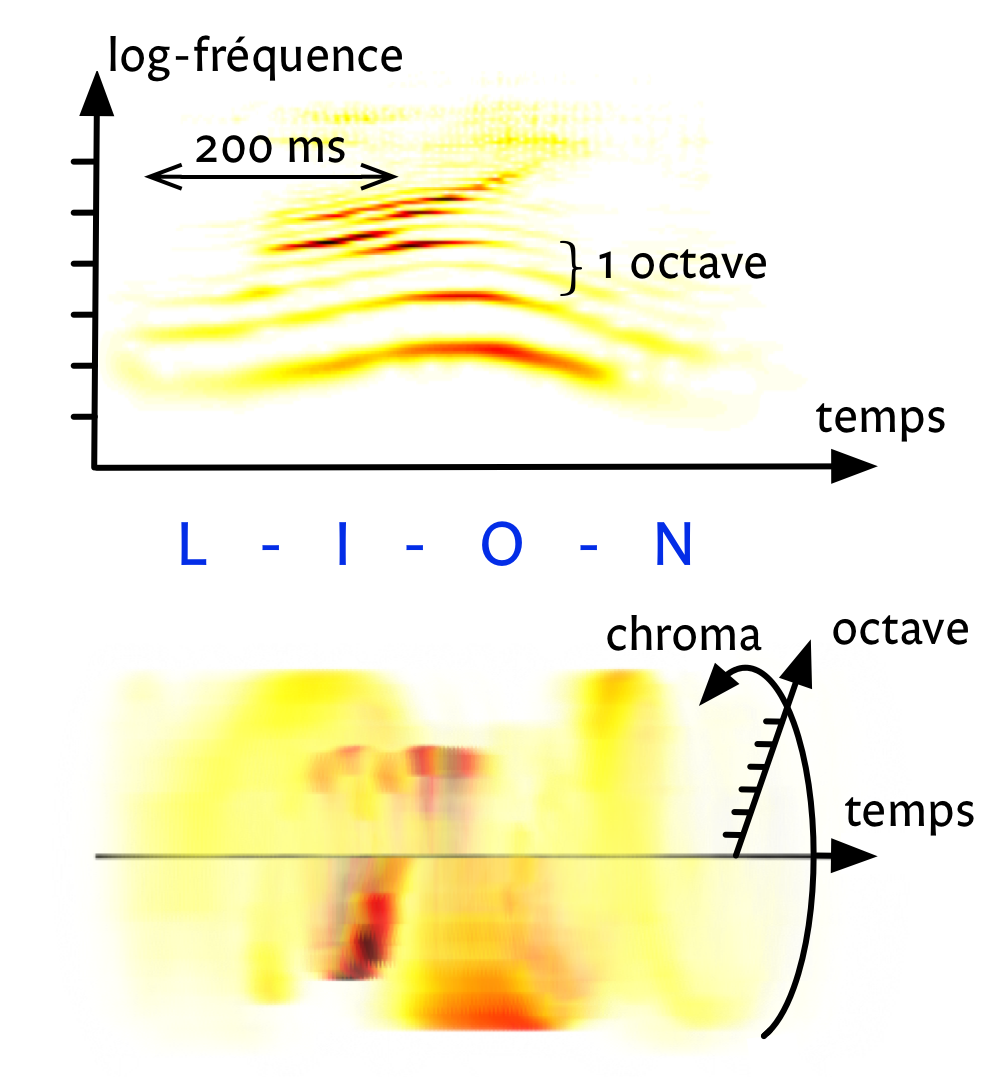
\includegraphics[width=8.8cm]{/Users/vlostan/GRETSI/figures/fig1/gretsi_fig1}\hfill{}

\protect\caption{En haut, un scalogramme du mot anglais \emph{lion}. En bas, le spiralogramme
correspondant : le temps est la coordonn\'{e}e longitudinale, le chroma
la coordonn\'{e}e angulaire, l'octave la coordonn\'{e}e radiale. Les
fr\'{e}quences aigues sont pr\`{e}s de l'axe longitudinal. La clart\'{e}
et la transparence sont inversement proportionelles \`{a} l'amplitude
des coefficients.\label{fig:spiralogram}}
\end{figure}



\section{Transform\'{e}es en ondelettes sur la spirale}

C'est en raison de ses bonnes propri\'{e}t\'{e}s de r\'{e}solution
temps-fr\'{e}quence, de stabilit\'{e} aux d\'{e}formations, et de
sparsit\'{e} que le scalogramme $x_{1}(u_{1},\lambda_{1})$ est un
outil de choix pour la classification de sons. Or, afin de pouvoir
g\'{e}n\'{e}raliser une classe de signaux \`{a} partir d'un nombre
limit\'{e} d'exemples, il est n\'{e}cessaire de construire une repr\'{e}sentation
invariante par translation \`{a} l'\'{e}chelle temporelle $T$ des
unit\'{e}s \`{a} classifier. Le scalogramme est une repr\'{e}sentation
\emph{covariante }\`{a} la translation, bien qu'on puisse le rendre
invariant en appliquant une moyenne glissante sur l'axe temporel.
L'\'{e}chelle $T$ vaut typiquement $200\,\mathrm{ms}$ pour des notes
de musique ou des syllabes ; pourtant, en raison de la nature transitoire
des signaux de musique et de parole, les capacit\'{e}s de discrimination
du scalogramme chutent d\`{e}s que $T$ d\'{e}passe $20\,\mathrm{ms}$.
Afin d'\'{e}tendre cette limite, il s'agit de d\'{e}moduler les oscillations
du scalogramme $x_{1}(u_{1},\lambda_{1})$ dont la p\'{e}riode est
inf\'{e}rieure \`{a} $T$ ; encore une fois, on requiert une bonne
stabilit\'{e} \`{a} la variabilit\'{e} naturelle des sons \`{a} l'int\'{e}rieur
d'une classe.

Compte tenu de ces observations, {[}And\'{e}n et Mallat, 2011{]} ont
introduit la transform\'{e}e de scattering pour les sons, comme le
\og scalogramme du scalogramme \fg{}. Pour toute fr\'{e}quence $\lambda_{1}$,
il s'agit de transformer $x_{1}(u_{1},\lambda_{1})$ en ondelettes
comme un signal unidimensionnel du temps $u_{1}$, et d'appliquer
le module :

\begin{equation}
x_{2}(u_{1},\lambda_{1},\lambda_{2})=\vert x_{1}(u_{1},\lambda_{1})\ast\psi_{\lambda_{2}}(u_{1})\vert,\label{eq:plain-scattering}
\end{equation}
o\`{u} $\psi_{\lambda_{2}}(u_{1})$ est une ondelette de fr\'{e}quence
centrale $\lambda_{2}$ (en Hertz). La transform\'{e}e de scattering
capture explicitement les modulations d'amplitude du signal, ce qui
a men\'{e} \`{a} des progr\`{e}s consid\'{e}rables en classification
de signaux. Cependant, elle n'est pas stable aux mouvement de hauteur
au-del\`{a} de $Q^{-1}$, soit typiquement un seizi\`{e}me d'octave.
Pour int\'{e}grer l'\'{e}volution de hauteur dans la transform\'{e}e,
on peut red\'{e}finir $x_{2}$ comme 
\[
x_{2}(u_{2},\lambda_{1},\lambda_{2})=\vert x_{1}\ast\psi_{\lambda_{2}}\vert(u_{2}),
\]
o\`{u} $u_{2}$ est une variable g\'{e}n\'{e}rique construite \`{a}
partir du temps $u_{1}$ et de la fr\'{e}quence $\lambda_{1}$. Il
faut remarquer que cette \'{e}quation est une g\'{e}n\'{e}ralisation
du mod\`{e}le original du scattering \ref{eq:plain-scattering} :
en \'{e}crivant $u_{2}=u_{1}$ et en factorisant l'action de $\psi_{\lambda_{2}}(u_{2})$
sur toutes les fr\'{e}quences $\lambda_{1}$, on parvient \`{a} $\vert x_{1}\ast\psi_{\lambda_{2}}\vert(u_{2})$. 

Le mod\`{e}le cortical de {[}Patil et al.{]} effectue des transform\'{e}es
sur les d\'{e}placements joints en temps et en log-fr\'{e}quence :
$u_{2}=(u_{1},\log_{2}\lambda_{1})$. La variable de Fourier correspondante
s'\'{e}crit $\lambda_{2}=(a,b)$ o\`{u} $a$ est la fr\'{e}quence
temporelle (en Hertz) $u_{1}$ et $b$ est la fr\'{e}quence log-fr\'{e}quentielle
(en cycles par octave). 
\[
\psi_{\lambda_{2}}(u_{1},\log_{2}\lambda_{1})=\psi_{a}(u_{1})\ast\psi_{b}(\log_{2}\lambda_{1})
\]
Nous proposons d'\'{e}tendre ce mod\`{e}le afin d'inclure la variabilit\'{e}
des d\'{e}placements sur les octaves. On pose donc $u_{2}=(u_{1},\log_{2}\lambda_{1},\lfloor\log_{2}\lambda_{1}\rfloor)$
la variable de d\'{e}placement sur la spirale. La variable de Fourier
correspondante s'\'{e}crit $\lambda_{2}=(a,b,c)$ o\`{u} $a$ est
la fr\'{e}quence temporelle (en Hertz), $b$ est la fr\'{e}quence
log-fr\'{e}quentielle (en cycles par octave), $c$ est la \og fr\'{e}quence
selon les octaves \fg{} (en cycles par octave). L'exp\'{e}rience
de Shepard nous apprend que, bien les fr\'{e}quences $b$ et $c$
soient exprim\'{e}es dans la m\^{e}me unit\'{e}, elles correspondent
\`{a} des ph\'{e}nom\`{e}nes diff\'{e}rents : avec typiquement $\vert b^{-1}\vert<1$
octave et $\vert c^{-1}\vert>1$ octave, $b$ quantifie un d\'{e}placement
angulaire sur la spirale tandis que $c$ quantifie un d\'{e}placement
radial. On propose d'appeler \og ondelettes de Shepard \fg{} les
produits s\'{e}parables d'ondelettes sur la spirale $u_{2}=(u_{1},\log_{2}\lambda_{1},\lfloor\log_{2}\lambda_{1}\rfloor)$
: 
\[
\psi_{\lambda_{2}}(u_{1},\log_{2}\lambda_{1},\lfloor\log_{2}\lambda_{1}\rfloor)=\psi_{a}(u_{1})\ast\psi_{b}(\log_{2}\lambda_{1})\ast\psi_{c}(\lfloor\log_{2}\lambda_{1}\rfloor).
\]
Sur la figure 2, on a repr\'{e}sent\'{e} deux ondelettes de Shepard
$\psi_{\lambda_{2}}$ pour diff\'{e}rentes valeurs de fr\'{e}quences
$a$, $b$ et $c$.

\begin{figure}
\hfill{}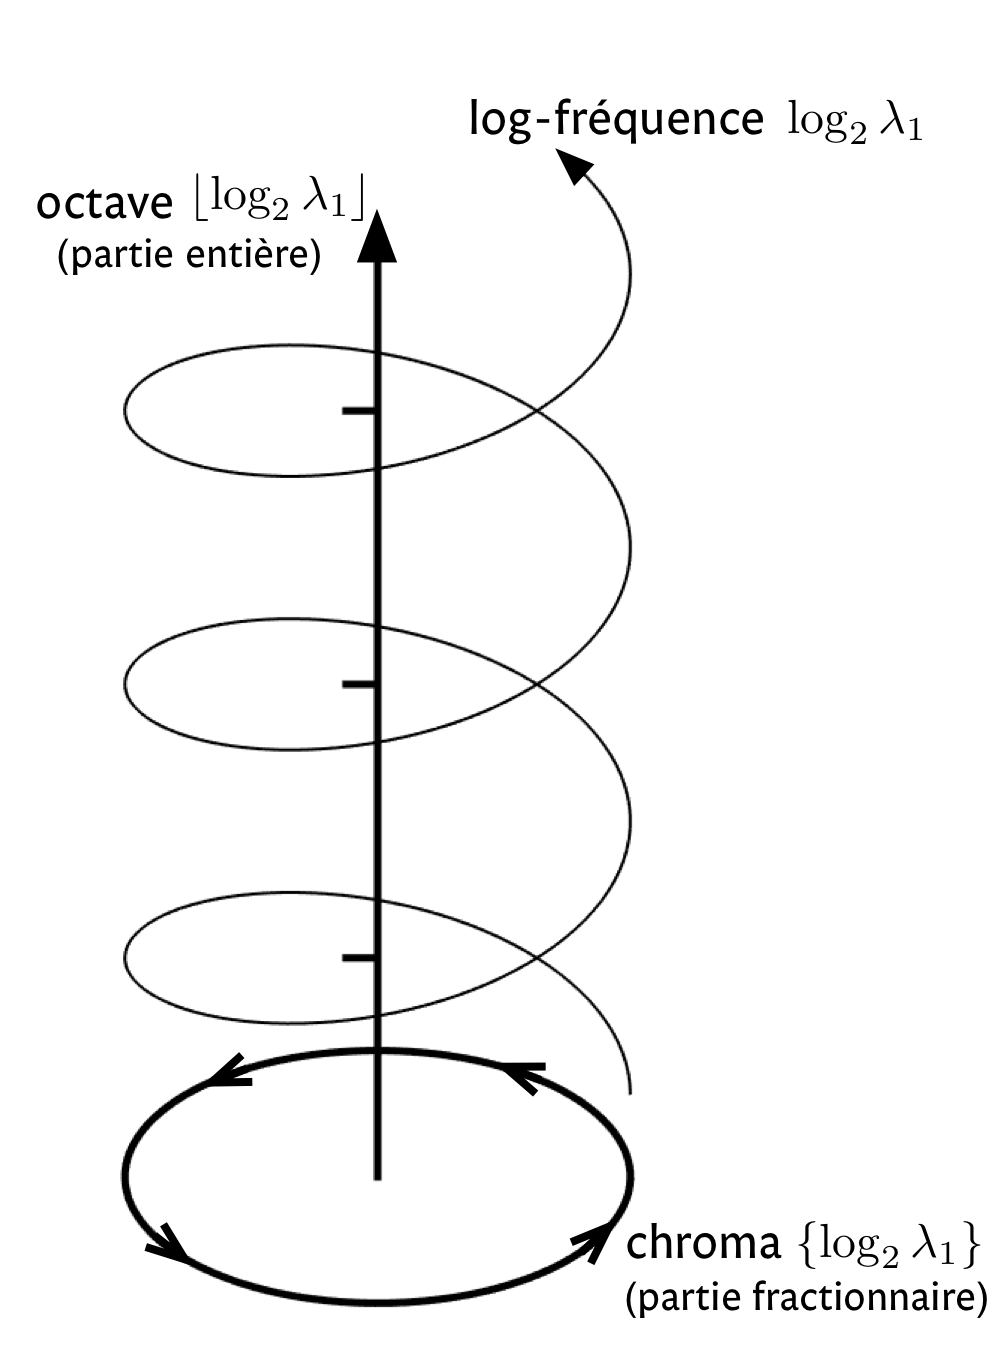
\includegraphics{/Users/vlostan/GRETSI/figures/fig2/v4/gretsi_fig2}\hfill{}

\protect\caption{Deux ondelettes en spirale $\psi_{\lambda_{2}}(u_{2})$ \'{e}tal\'{e}es
sur le plan temps-fr\'{e}quence, pr\'{e}sentant des $\lambda_{2}=(a,b,c)$
diff\'{e}rents et une localisation temps-fr\'{e}quence diff\'{e}rente.
\`{A} gauche : $a^{-1}=120\,\mathrm{ms}$, $b^{-1}=-0.25\,\mathrm{octave}$,
$c^{-1}=+2\,\mathrm{octaves}$. \`{A} droite : $a^{-1}=60\,\mathrm{ms}$,
$b^{-1}=+0.5\,\mathrm{octave}$, $c^{-1}=-4\,\mathrm{octaves}$. On
a affich\'{e} la partie r\'{e}elle des coefficients. Le noir correspond
\`{a} des coefficients positifs et le blanc \`{a} des coefficients
n\'{e}gatifs.}
\end{figure}


\begin{figure}
\hfill{}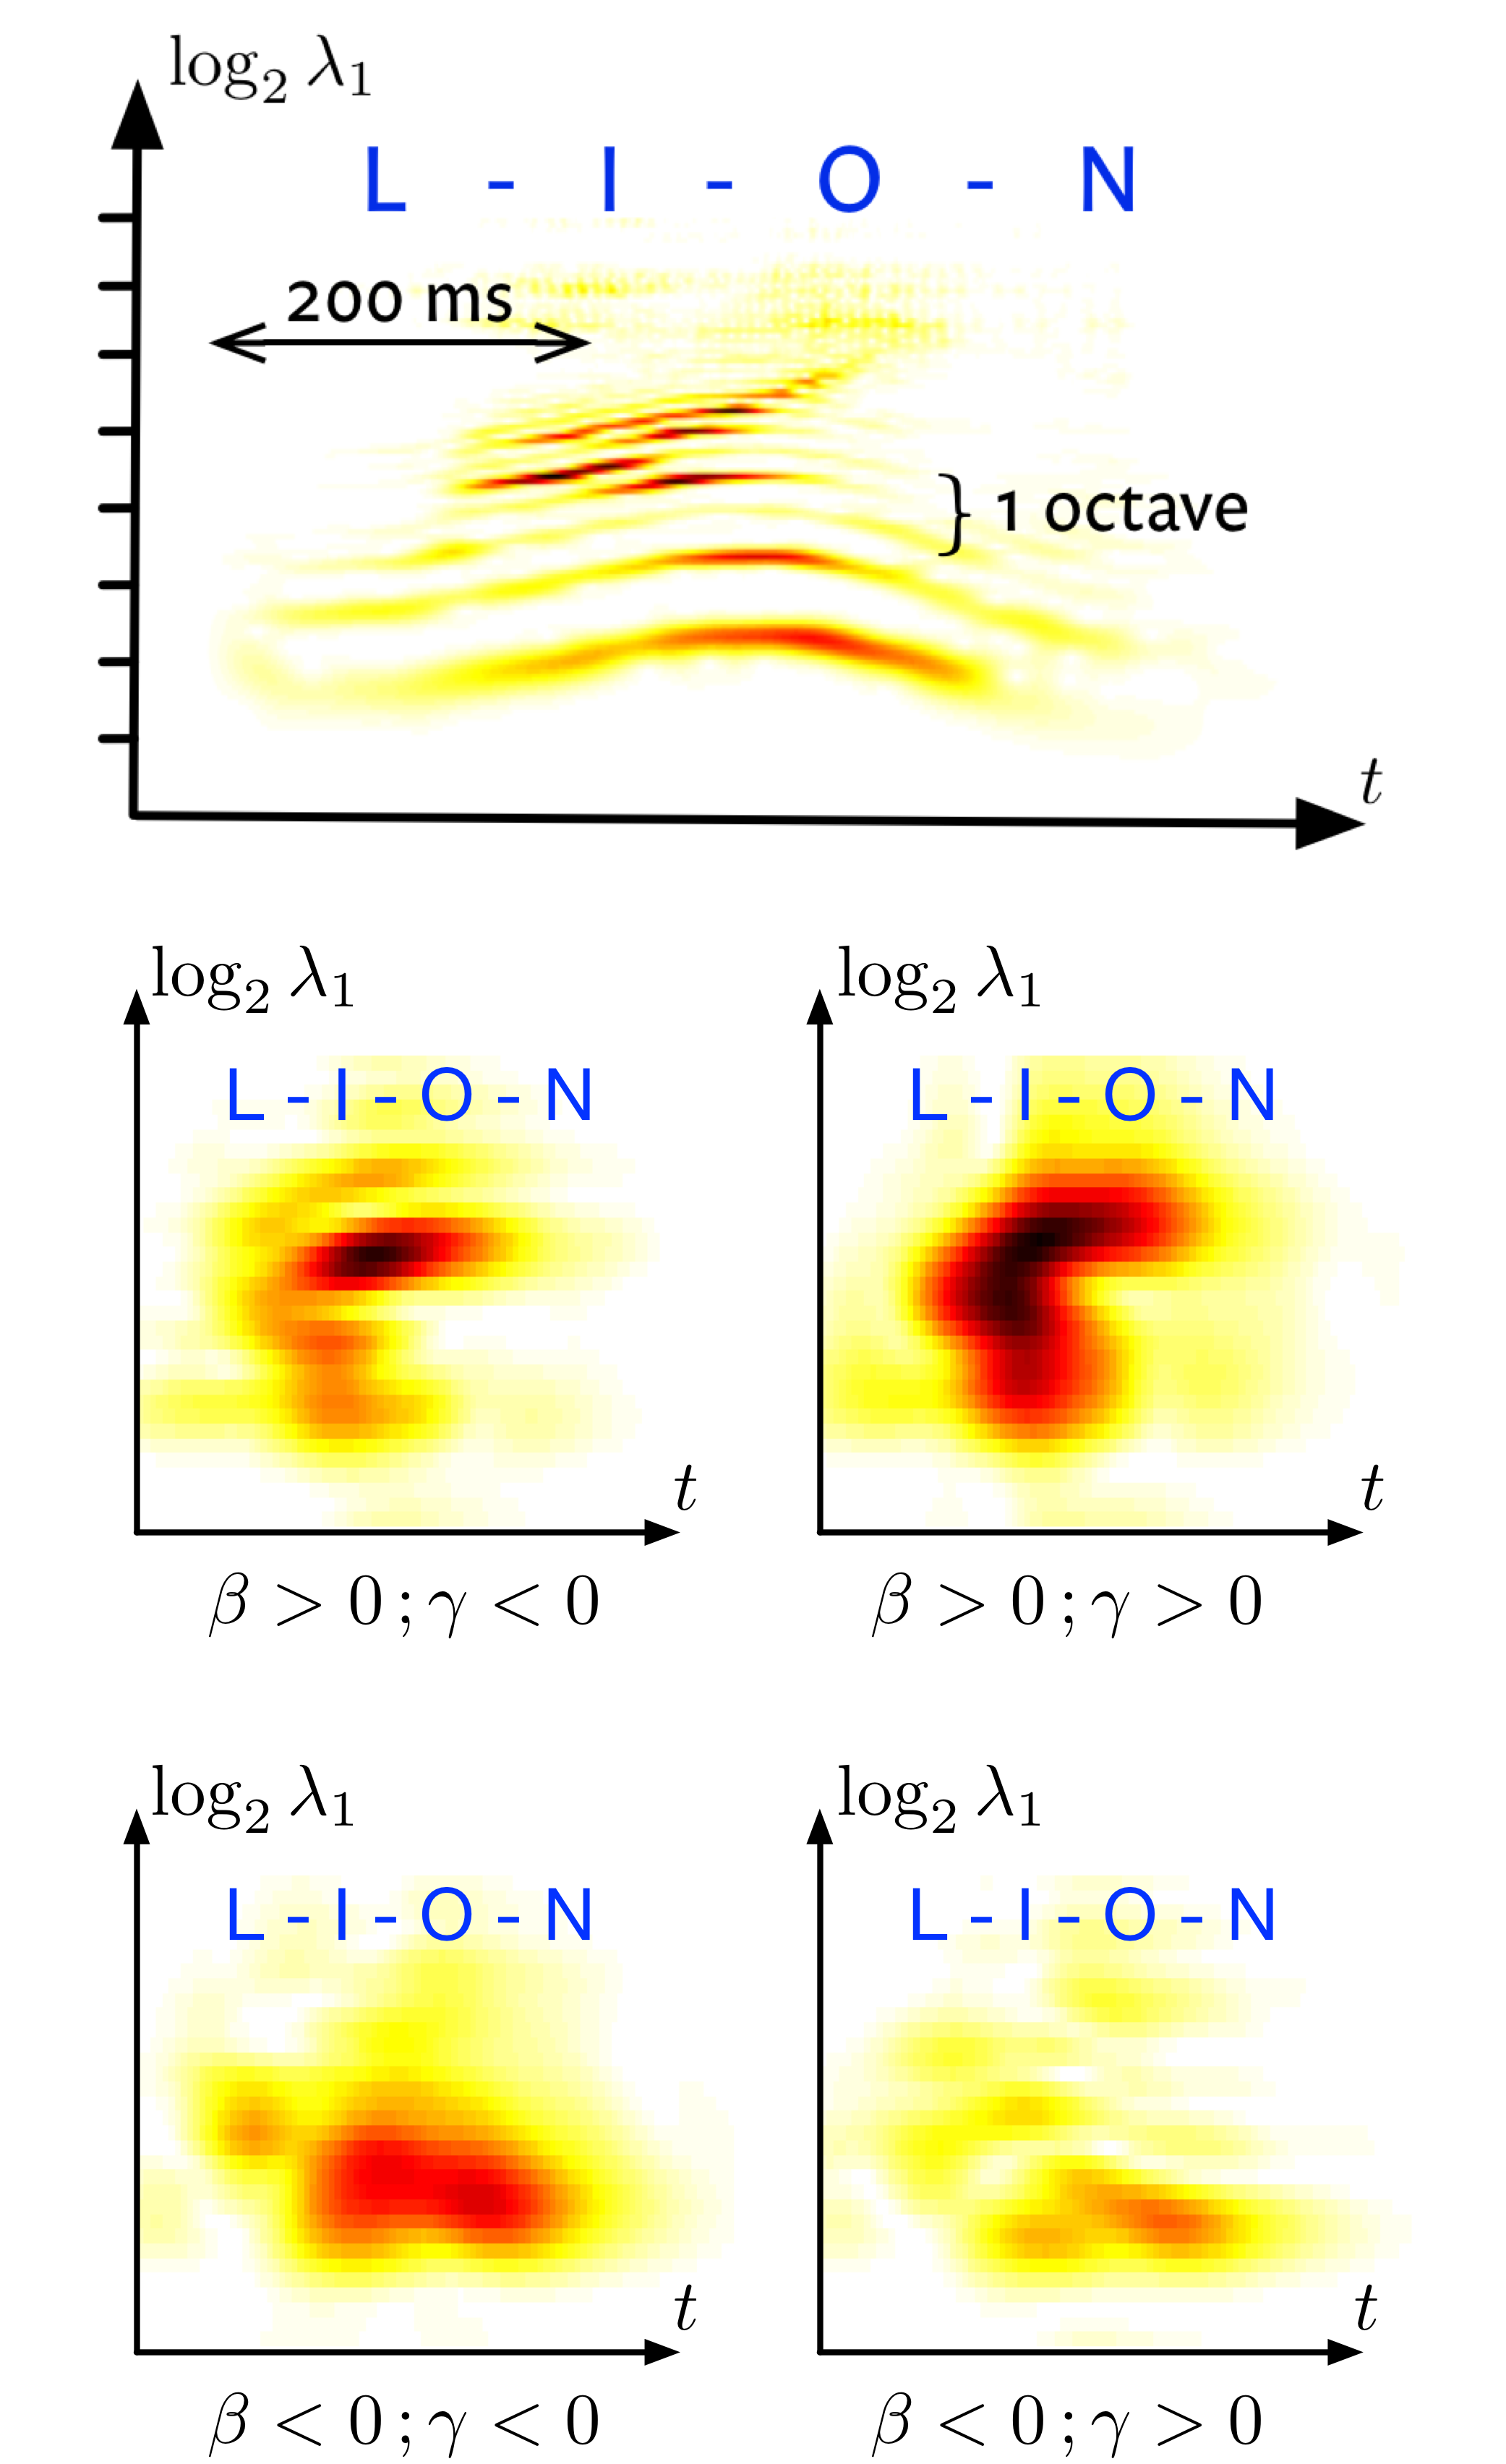
\includegraphics{/Users/vlostan/GRETSI/figures/fig3/gretsi_fig3}\hfill{}

\protect\caption{Coefficients de scattering de $x_{2}(u_{1},\lambda_{1},\lambda_{2})$
en fonction du temps $u_{1}$ et de la log-fr\'{e}quence $\log_{2}\lambda_{1}$,
pour $\lambda_{2}=(a,b,c)$ fix\'{e} avec $a^{-1}=120\,\mathrm{ms}$,
$b^{-1}=\pm1\,\mathrm{octave}$, $c^{-1}=\pm4\,\mathrm{octaves}$.
On constate que la syllabe /\textprimstress lai/ active en particulier
les coefficients tels que $b>0$, $c>0$ (hauteur montante, timbre
montant) tandis que /\textsci \textschwa n/ active les coefficients
tels que $b<0$, $c<0$ (hauteur descendante, timbre descendant).
La clart\'{e} est inversement proportionelle \`{a} l'amplitude des
coefficients.}
\end{figure}



\section{D\'{e}formations du mod\`{e}le source-filtre}

Soient

\[
e(t)=\sum_{k=1}^{K}\exp(\mathrm{i}k\xi t)
\]
un signal harmonique \og source \fg{} et $t\mapsto\mu(t)$ un diff\'{e}omorphisme
du temps ; on d\'{e}finit $e_{\mu}(t)=(e\circ\mu)(t)$ la source d\'{e}form\'{e}e.
De m\^{e}me, on part d'un \og filtre \fg{} $h(t)$ et d'un diff\'{e}omorphisme
$t\mapsto\nu(t)$ pour d\'{e}finir $h_{\nu}(t)=(h\circ\nu)(t)$. Le
mod\`{e}le source-filtre d\'{e}form\'{e} est le signal $x(t)=[e_{\mu}\ast h_{\nu}](t)$.
Dans cette section, on note $\eta$ la fr\'{e}quence centrale en Hertz
de l'ondelette $\psi(t)$, de sorte que la r\'{e}solution $\lambda_{1}$
est maintenant une grandeur sans dimension.
\begin{lem*}
Pour tout $\lambda_{1}$ tel que 
\begin{enumerate}
\item $\Vert\ddot{\nu}/\dot{\nu}\Vert_{\infty}\ll\lambda_{1}\eta/Q$ (filtre
lentement variable) et
\item $\Vert\dot{\hat{h}}/\hat{h}\Vert_{\infty}\Vert1/\dot{\nu}\Vert_{\infty}\ll Q\eta^{-1}/\lambda_{1}$
(profil spectral r\'{e}gulier),
\end{enumerate}
la transform\'{e}e en ondelettes $[h_{\nu}\ast\psi_{\lambda_{1}}]$
se factorise en

\[
[h_{\nu}\ast\psi_{\lambda_{1}}](t)\approx H(\log_{2}\lambda_{1}-\log_{2}\dot{\nu}(t))\psi_{\lambda_{1}}\left(\dfrac{\nu(t)}{\dot{\nu}(t)}\right)
\]
o\`{u} $H(\log_{2}\lambda_{1})=\lambda_{1}\hat{h}(\lambda_{1}\eta)$.\end{lem*}
\begin{proof}
Gr\^{a}ce \`{a} la premi\`{e}re hypoth\`{e}se, on d\'{e}veloppe $\nu(t-u)\approx\nu(t)-\dot{\nu}(t)\times u$
sur le support de $\psi_{\lambda_{1}}(t)$. Le changement de variable
$u^{\prime}=\dot{\nu}(t)\times u$ conduit \`{a}
\[
[h_{\nu}\ast\psi_{\lambda_{1}}](t)=\int_{\mathbb{R}}h(\nu(t)-u^{\prime})\psi_{\lambda_{1}}\left(\dfrac{u^{\prime}}{\dot{\nu}(t)}\right)\,\dfrac{\mathrm{d}u^{\prime}}{\dot{\nu}(t)}.
\]
L'ondelette $\psi_{\lambda_{1}}$ v\'{e}rifiant $\psi_{\lambda_{1}}(\dot{\nu}(t)^{-1}u^{\prime})=\dot{\nu}(t)\psi_{\dot{\nu}(t)^{-1}\lambda_{1}}(u^{\prime})$,
on peut convertir le facteur de dilatation $\dot{\nu}(t)$ en une
transposition fr\'{e}quentielle. D'o\`{u} $[h_{\nu}\ast\psi_{\lambda_{1}}](t)=[h\ast\psi_{\dot{\nu}(t)^{-1}\lambda_{1}}](t)$,
ce qui s'\'{e}crit comme un produit dans le domaine de Fourier :
\[
[h_{\nu}\ast\psi_{\lambda_{1}}](t)=\dfrac{1}{2\pi}\int_{\mathbb{R}}\hat{h}(\omega)\hat{\psi}_{\dot{\nu}(t)^{-1}\lambda_{1}}(\omega)\exp(\mathrm{i}\omega\nu(t))\,\mathrm{d}u^{\prime}.
\]
Gr\^{a}ce \`{a} la seconde hypoth\`{e}se, on approxime localement
$\hat{h}(\omega)$ par la constante $\hat{h}(\dot{\nu}(t)^{-1}\lambda_{1})$
sur le support fr\'{e}quentiel de $\hat{\psi}_{\dot{\nu}(t)^{-1}\lambda_{1}}$.
D\`{e}s lors, l'int\'{e}grale ci-dessus peut \^{e}tre vue comme la
transform\'{e}e de Fourier inverse de $\hat{\psi}_{\dot{\nu}(t)^{-1}\lambda_{1}}(\omega)$
\'{e}valu\'{e}e en $\nu(t)$. On conclut en revenant \`{a} l'ondelette
$\psi_{\lambda_{1}}$ avec l'\'{e}quation $\dot{\nu}(t)^{-1}\psi_{\dot{\nu}(t)^{-1}\lambda_{1}}(\nu(t))=\psi_{\lambda_{1}}(\nu(t)/\dot{\nu}(t))$.\end{proof}
\begin{prop*}
Soit $\lambda_{1}$ de la forme $k\xi\eta^{-1}$, avec $k\leq K$.
Si les conditions suivantes sont v\'{e}rifi\'{e}es :
\begin{enumerate}
\item $\Vert\ddot{\nu}/\dot{\nu}\Vert_{\infty}\ll\lambda_{1}\eta/Q$ (filtre
lentement variable),
\item $\Vert\dot{\hat{h}}/\hat{h}\Vert_{\infty}\Vert1/\dot{\nu}\Vert_{\infty}\ll Q\eta^{-1}/\lambda_{1}$
(r\'{e}ponse fr\'{e}quentielle r\'{e}guli\`{e}re),
\item $\Vert\ddot{\mu}/\dot{\mu}\Vert_{\infty}\ll\lambda_{1}\eta/Q$ (source
lentement variable) et
\item $k<Q/2$ (partiel de rang faible),
\end{enumerate}
alors le module de la transform\'{e}e en ondelettes du mod\`{e}le
source-filtre d\'{e}form\'{e}

\[
\vert e_{\alpha}\ast h_{\beta}\ast\psi_{\lambda_{1}}\vert(t)\approx E(\log_{2}\lambda_{1}-\log_{2}\dot{\mu}(t))H(\log_{2}\lambda_{1}-\log_{2}\dot{\nu}(t))
\]
est localement s\'{e}parable en une r\'{e}ponse de source $E(\log_{2}\lambda_{1})=\vert\widehat{\psi_{\lambda_{1}}}(k\xi)\vert$
et une r\'{e}ponse de filtre $H(\log_{2}\lambda_{1})=\lambda_{1}\hat{h}(\lambda_{1}\eta)$,
chacune en mouvement rigide sur l'axe log-fr\'{e}quentiel $\log_{2}\lambda_{1}$;
le mouvement de $E$ (resp. $H$) \'{e}tant r\'{e}gi par le signal
$\log_{2}\dot{\mu}(t)$ (resp. $\log_{2}\dot{\nu}(t))$.\end{prop*}
\begin{proof}
On part des hypoth\`{e}ses (a) et (b) pour affirmer le lemme pr\'{e}c\'{e}dent
:
\[
\left[e_{\mu}\ast h_{\nu}\ast\psi_{\lambda_{1}}\right](t)=H\left(\log_{2}\lambda_{1}-\log_{2}\dot{\nu}(t)\right)\times\int_{\mathbb{R}}e_{\mu}(t-u)\psi_{\lambda_{1}}\left(\dfrac{\nu(u)}{\dot{\nu}(u)}\right)\,\mathrm{d}u.
\]


Comme dans la preuve du lemme, on pose $u^{\prime}=\dot{\mu}(t)\times(\frac{\nu(t)}{\dot{\nu}(t)}+u-t)$,
on d\'{e}veloppe et simplifie $\frac{\nu(u)}{\dot{\nu}(u)}\approx\frac{u^{\prime}}{\dot{\mu}(t)}$,
et l'on convertit la dilatation temporelle en transposition fr\'{e}quentielle
avec l'\'{e}quation $\dot{\mu}(t)^{-1}\psi_{\lambda_{1}}(\dot{\mu}(t)^{-1}u^{\prime})=\psi_{\dot{\mu}(t)^{-1}\lambda_{1}}(u^{\prime})$
:
\[
\begin{array}{c}
\int_{\mathbb{R}}e_{\mu}(t-u)\psi_{\lambda_{1}}\left(\frac{\nu(u)}{\dot{\nu}(u)}\right)\,\mathrm{d}u\\
=\int_{\mathbb{R}}e_{\mu}\left(\frac{\nu(t)}{\dot{\nu}(t)}-\frac{u^{\prime}}{\dot{\mu}(t)}\right)\psi_{\dot{\mu}(t)^{-1}\lambda_{1}}(u^{\prime})\,\mathrm{d}u^{\prime}
\end{array}
\]
Avec l'hypoth\`{e}se (3), on lin\'{e}arise le diff\'{e}omorphisme
$\mu$ autour de $\frac{\nu(t)}{\dot{\nu}(t)}$, ce qui permet de
voir l'int\'{e}grale ci-dessus comme la convolution $[e\ast\psi_{\dot{\mu}(t)^{-1}\lambda_{1}}]$
\'{e}valu\'{e}e en $\mu(\frac{\nu(t)}{\dot{\nu}(t)})$. Puisque le
banc de filtres a un facteur de qualit\'{e} constant $Q$, la largeur
de bande \`{a} la fr\'{e}quence $k\xi\dot{\mu}(t)$ est $k\xi\dot{\mu}(t)Q^{-1}$.
L'hypoth\`{e}se (4) peut se r\'{e}\'{e}crire $(k+1)\xi\dot{\mu}(t)>k\xi\dot{\mu}(t)+\frac{k\xi\dot{\mu}(t)}{2Q}$
; autrement dit, le $(k+1)^{\text{\`{e}me}}$ partiel est hors de
la bande passante de $\psi_{\dot{\mu}(t)\lambda_{1}}$. Plus g\'{e}n\'{e}ralement,
les partiels $k^{\prime}\neq k$ ont une contribution n\'{e}gligeable
\`{a} la transform\'{e}e en ondelettes de $e(t)$. En l'absence d'interf\'{e}rences,
le module $\vert e\ast\psi_{\dot{\mu}(t)^{-1}\lambda_{1}}\vert(t)$
se r\'{e}sume au seul terme $E(\log_{2}\lambda_{1}-\log_{2}\dot{\mu}(t))$
o\`{u} l'on a d\'{e}fini $E(\log_{2}\lambda_{1})=\vert\widehat{\psi_{\lambda_{1}}}(k\xi)\vert$
sur un axe log-fr\'{e}quentiel.
\end{proof}
On peut calculer explicitement la r\'{e}ponse de source dans le cas
d'un spectre harmonique : 
\[
E(\log_{2}\lambda_{1})=\sum_{k=1}^{K}\delta(\log_{2}(\lambda_{1})-\log_{2}(k\xi\eta^{-1})).
\]
Soit $n\in\mathbb{N}$; pourvu que $\lambda_{1}=k\xi\eta^{-1}$ soit
tel que $k<2^{-n}K$, on retrouve un partiel $n$ octaves exactement
au-dessus de la fr\'{e}quence $\lambda_{1}$ : d'o\`{u} $E(\log_{2}\lambda_{1}+n)=E(\log_{2}\lambda_{1})$.
Par ailleurs, les hypoth\`{e}ses (b) et (c) permettent d'\'{e}crire
$H(\log_{2}\lambda_{1})\approx H(\log_{2}\lambda_{1}+\Delta)$ pour
toute d\'{e}viation de chroma $\Delta$. Ce r\'{e}sultat sugg\`{e}re
qu'il est possible de s\'{e}parer les fonctions $\log_{2}\dot{\alpha}(t)$
et $\log_{2}\dot{\beta}(t)$ en d\'{e}composant leurs trajectoires
sur les couples de variables temps-chroma et temps-octave.


\begin{thebibliography}{1}
\bibitem{AM11}J. And\'{e}n, S. Mallat. Deep Scattering Spectrum.
\emph{IEEE Transactions on Signal Processing}, vol. 62, n\textdegree{}
16, p. 4114\textendash 4128, 2014.

\bibitem{Fla01}P. Flandrin. Time-frequency and chirps. In\emph{ Proc.
SPIE Meeting Wavelet Applications VIII}, vol. 4391, p. 161\textendash 175,
Orlando (FL), 2001.

\bibitem{Mal00}S. Mallat. \emph{Une exploration des signaux en ondelettes}.
Les \'{E}ditions de l'\'{E}cole polytechnique, 2000.

\bibitem{Ris78} J.-C. Risset. Paradoxes de hauteur. Rapport Ircam
11/78, 1978.

\bibitem{PPS+12}K. Patil, D. Pressnitzer, S. Shamma, M. Elhilali.
Music in our ears: the biological bases of musical timbre perception.
\emph{PLoS computational biology}, vol. 8, n\textdegree{} 11, 2012.

\bibitem{WUP+99}J. D. Warren, S. Uppenkamp, R. D. Patterson, T. Griffiths.
Separating pitch chroma and pitch height in the human brain. \emph{Proceedings
of the National Academy of Sciences}, vol. 100, n\textdegree{} 17,
p. 10038\textendash 10042, 2003.\end{thebibliography}

\end{document}
